\documentclass[conference]{IEEEtran}
\IEEEoverridecommandlockouts
% The preceding line is only needed to identify funding in the first footnote. If that is unneeded, please comment it out.
\usepackage{cite}
\usepackage{amsmath,amssymb,amsfonts,amsthm}
\usepackage{algorithmic}
\usepackage{graphicx}
\usepackage{textcomp}
\usepackage{xcolor}
\usepackage{colortbl}
\usepackage{stfloats}
\usepackage{cite}  % converts [1],[2] to [1,2]
\usepackage{multicol}
\usepackage{hyperref}


\makeatletter
\def\@citex[#1]#2{\leavevmode
\let\@citea\@empty
\@cite{\@for\@citeb:=#2\do
{\@citea\def\@citea{,\penalty\@m\ }%
\edef\@citeb{\expandafter\@firstofone\@citeb\@empty}%
\if@filesw\immediate\write\@auxout{\string\citation{\@citeb}}\fi
\@ifundefined{b@\@citeb}{\hbox{\reset@font\bfseries ?}%
\G@refundefinedtrue
\@latex@warning
{Citation `\@citeb' on page \thepage \space undefined}}%
{\@cite@ofmt{\csname b@\@citeb\endcsname}}}}{#1}}
\makeatother

\renewcommand{\qedsymbol}{$\blacksquare$}

\newtheorem{thm}{Theorem}[section]
\newtheorem{lem}[thm]{Lemma}
\newtheorem{prop}[thm]{Proposition}
\newtheorem{cor}{Corollary}
\newtheorem{conj}{Conjecture}[section]
\theoremstyle{definition}
\newtheorem{defn}{Definition}[section]
\newtheorem{exmp}{Example}[section]
\newtheorem{rem}{Remark}

\def\BibTeX{{\rm B\kern-.05em{\sc i\kern-.025em b}\kern-.08em
    T\kern-.1667em\lower.7ex\hbox{E}\kern-.125emX}}
    
\begin{document}
\title{Finitely Presented Group Construction from Turing Machine}

\author{\IEEEauthorblockN{Max Shamray}
\IEEEauthorblockA{\textit{Saint Petersburg State University}\\
St. Petersburg, Russia \\
vortmanmax@gmail.com}
\and
\IEEEauthorblockN{Semyon Grigorev}
\IEEEauthorblockA{\textit{Saint Petersburg State University}\\
\textit{JetBrains Research}\\
St. Petersburg, Russia \\
s.v.grigoriev@spbu.ru \\
semyon.grigorev@jetbrains.com}
}

\maketitle

\begin{abstract}
A study of formal languages showed there are open problems that we can’t solve involving traditional methods. In this paper, we try to bring a group theory methods into play by implementing an algorithm for constructing a finitely presented group from a Turing machine, which described by Sapir, Birget, and Rips. Also, we obtained an injective mapping from an alphabet of the Turing machine language into a word problem of the corresponding group. This algorithm can be used to further study the classification of formal languages ​​in terms of well-known classes of groups, highlight signs of belonging to a particular class and apply the algebraic methods to formal languages.
\end{abstract}

\begin{IEEEkeywords}
Turing machine, group theory, word problem, formal languages
\end{IEEEkeywords}

\section{Introduction}

Formal languages are the theoretical foundation of system programming, 
namely the development of translators and static analyzers, through lexical, 
syntactic and semantic analysis. 
The formal language analysis approach has begun new development in the 50s of the last century \cite{chomsky1, chomsky2}. 
During this time, it found application not only in areas directly 
related to programming but, among other things, in the analysis of graph data models, 
which are used \cite{Hellings2015QueryingFP, Azimov2017ContextfreePQ}, 
for example, in bioinformatics and social networks.

Development entails new theoretical problems and challenges. 
Several of them are associated with the advent of conjunctive and Boolean language classes. 
The first and most important issue concerns the restriction of Boolean grammars.
The limitations of the expressive power of conventional context-free grammars are fairly well known. There are direct methods for proving the unrepresentability of certain languages, 
such as the pumping lemma and its variants, which show that some languages 
cannot be generated by a context-free grammar. On the contrary, there are no methods 
for proving the unrepresentability of languages by Boolean grammars, and this 
is the main gap in the knowledge of these grammars. Similarly, 
such methods are not known for conjunctive grammars \cite{OKHOTIN201327}.

Recently, there has been a tendency to shift the direction of methods of studying formal languages.
Researchers are moving away from combinatorial techniques to more mathematically oriented disciplines.
One of the possible directions is the study of formal languages with the help of 
a group-theoretical methods.

Well known that formal languages too close to group theory. 
It is seen if we pay attention to a group constructed using an alphabet of 
formal language like generators set and concatenation operation. Moreover, 
there is a word problem with several statements that have been already 
proved to show the algebraic properties of groups correspond to the properties of formal languages. 
For example, for a finitely generated group, the following is true:
\begin{itemize}
    \item Word problem for $G$ is solvable $\iff W(G)$ --- recursive language. 
    \item $W(G)$ --- regular $\iff G$ --- finite \cite{Anisimov}.
    \item $W(G)$ --- context-free $\iff \exists H < G$ --- finite index \cite{Muller}.
\end{itemize}
Unfortunately, there is no easy way to build a group from a formal language. 
For this, complex mathematical transformations are carried out for a Turing machine 
that recognizes a language, and it is not advisable to produce them with a pen and paper, 
but studying the group properties of languages seems to be a rather promising 
area of research \cite{Sapir, SpaceFunc}.
Thus, the problem of the algorithmization algorithm 
for constructing a group using a Turing machine is actual.
Besides, the question of studying the group properties of language classes 
such as conjunctive and Boolean remains open. 

In total, the main contribution of this work is the implementation of an algorithm invented by Sapir, Birget, and Rips \cite{Sapir}, which is constructing a finite presentation of a group by Turing machine.

\section{Background}
\subsection{Formal languages}

In this work, we use a standard definition for the formal languages such can be seen
for example in Chomsky's works (e.g. see \cite{chomsky1, chomsky2}).
In follows, we present the base ones we use in this work. 
Also, we touched the problem of conjunctive and Boolean languages, 
the definitions of which are given in this section
and can be seen in Okhotin's work \cite{OKHOTIN201327}. 

\begin{defn}
In the classic formalization a formal grammar G can be presented as four-tuple 
$G = (\Sigma, N, R, S)$ and consists of the following components:
\begin{itemize}
    \item A finite set $\Sigma$ of terminal symbols.
    \item A finite set $N$ of nonterminal symbols that is disjoint from $\Sigma$.
    \item A finite set $R$ of production rules, each rule of the form
    $(\Sigma \cup N)^{*}N(\Sigma \cup N)^{*} \to (\Sigma \cup N)^{*}$
    \item A letter S is the start nonterminal.
\end{itemize}
\end{defn}

\begin{defn}
A conjunctive grammar $G$ is a formal grammar with the special rule 
of the form 
$\\A \to \alpha_{1}\And \ldots \And \alpha_{m}$ where 
\begin{itemize}
    \item $A$ is a nonterminal.
    \item $\alpha_{i} \in (\Sigma \cup N)^*$.
\end{itemize}
Informally, such a rule asserts that every string $\omega$ over $\Sigma$ that satisfies each of the conditions represented by $\alpha _{1}, \dots, \alpha _{m}$, therefore, satisfies the condition defined by $A$.
\end{defn}

\begin{defn}
A Boolean grammar $G$ is a formal grammar with the special rule of the form 
$\\A\to \alpha_{1}\And \ldots \And \alpha_{m}\And \lnot \beta_{1}\And \ldots \And \lnot \beta_{n}$ where 
\begin{itemize}
    \item $A$ is a nonterminal.
    \item $m+n\geq 1$
    \item $\alpha_{1}, \dots, \alpha_{m}, \beta_{1}, \dots, \beta_{n} \in (\Sigma \cup N)^*$
\end{itemize}
Informally, such a rule asserts that every string $\omega$ over $\Sigma$ 
that satisfies each of the conditions represented by $\alpha_{1}, \dots, \alpha_{m}$
and none of the conditions represented by $\beta_{1}, \dots, \beta_{n}$, 
therefore, satisfies the condition defined by $A$.
\end{defn}

\begin{defn}
A recursively enumerable language is a formal language for which there exists a Turing machine 
(or other computable function) that will halt and accept when presented with any string 
in the language as input but may either halt and reject or loop forever when presented 
with a string, not in the language. Recursively enumerable languages are known as type-0 
languages in the Chomsky hierarchy of formal languages.
\end{defn}

\begin{defn}
A context-free grammar is a special case of a formal grammar 
(type 2 according to the Chomsky hierarchy), in which the left parts of all 
products are single non-terminals.
\end{defn}

\begin{defn}
A pushdown automaton is a finite state machine that has additional stack storage. The transitions a machine makes are based not only on the input and current state but also on the stack. The formal definition is defined as seven-tuple:
$M=(Q,\Sigma ,\Gamma ,\delta ,q_{0},Z,F)$ where
\begin{itemize}
    \item $Q$ is a finite set of states.
    \item $\Sigma$ is a finite set which is called the input alphabet.
    \item $\Gamma$ is a finite set which is called the stack alphabet.
    \item $\delta$ is a finite subset of ($Q \times (\Sigma \cup \{\varepsilon \})\times \Gamma) \times (Q\times \Gamma^{*})$, the transition relation.
    \item $q_{0}\in Q$ is the start state.
    \item $Z\in \Gamma$ is the initial stack symbol.
    \item $F\subseteq Q$ is the set of accepting states.
\end{itemize}
\end{defn}

\begin{thm} \label{thmpda}
Non-deterministic pushdown automata recognize exactly the context-free languages.
\end{thm}

\subsection{Group theory}

In this subsection, we going to define a free group, a group presentation,
a word problem, and several basic group theory definitions and theorems leading to it. 

\begin{defn}
A set G with an operation ($\cdot$) given on it is called a group if $\forall a, b, c \in G$ 
the following is true:
\begin{itemize}
\item $(a \cdot b) \cdot c = a \cdot (b \cdot c)$
\item $\exists e \in G : a \cdot e = e \cdot a = a$
\item $\exists a^{-1} : a \cdot a^{-1} = a^{-1} \cdot a = e$
\end{itemize}
\end{defn}

In group theory, cosets are divided according to the position of a group element 
into right and left cosets. For example, left coset can be defined as $aH = \{ ah : h \in H \}$
where $a \in G$, $H$ is subgroup of G.
A subgroup $H$ of a group $G$ is called normal if and only if for all 
elements $a$ of $G$ the corresponding left and right coset are equal, 
that is, $aH= Ha$. Furthermore, the cosets of $H$ in $G$ form a group 
called the quotient group or factor group. 

Normal closure $S^G$ of a subset $S$ of a group $G$ is the smallest normal subgroup 
of a group $G$ that contains the subset $S$.
\begin{equation}
    S^G = \{ gsg^{-1} : g \in G,\, s \in S \}
\end{equation}

\begin{thm}
The Fundamental Homomorphism Theorem.
The following result is one of the central results in group theory. 
If $\phi: G \to H$ is a homomorphism, then $Im(\phi) \cong G/Ker(\phi)$.
\end{thm}

Let $A = \{ a \}$ then $A^{-1} = \{ a^{-1} : a \in A \}$ and $A \cup A^{-1}$ is a group alphabet.
$\omega$ is word in alphabet $A \cup A^{-1}$ if and only if $\omega = a_1 \dots a_n$ 
where $a_i \in A \cup A^{-1}$ $\forall i$ from $1$ to $n$. 
The word is reducible if there is $i$ and letters $x_i$ and $x_{i+1}$ are mutually inverse. 

\begin{defn}
The set $G(A)$ of all irreducible words in the alphabet $A \cup A^{-1}$ 
is a group for the concatenation operation followed by reduction and is called free group. 
\end{defn}

Since in any group one can choose some system of generators $\{ g_i \}$ then there 
is a surjective homomorphism $\phi: G(A) \to G$ such that $\phi(a_i) = g_i$ 
where $\{a_i\} = A$. And by applying the fundamental homomorphism theorem 
($G \cong G(A)/Ker(\phi)$) we turn to the possibility of defining every group
as a factor of a group of a free group by some normal subgroup of it. 
In this regard, interesting methods for specifying a normal subgroup in a free group.

To define the equivalence relation in the words of a free group $G(A)$
let describe elementary transformations of words that do not change 
a coset of a word in a subgroup $R^{G(A)}$ where $R$ is a subset of $G(A)$ as follows:
\begin{enumerate}
\item Reduction.
\item Replacing the word $\omega = \omega_1 r^{\pm} \omega_2$ where $r \in R$ with the word $\omega_1 \omega_2$ and vice versa.
\end{enumerate}
Then the words $\omega_1$ and $\omega_2$ are equivalent if we can bring one to 
the other with the help of these transformations.

\begin{defn}
Set of relations $\{ r=1: r \in R \}$ is called determining for the group 
$G= \langle g_i \rangle$ if any other relation between 
$g_i$ follows from the system $\{ r=1 : r \in R \}$. If relations 
$\{ r=1 : r \in R \}$ is determining for the group $G$ then $G \cong G(A)/R^{G(A)}$ 
and then we can say that $G$ has a presentation $\langle A ~|~ R \rangle$.
\end{defn}

\begin{defn}
Word problem \eqref{eqwordproblem} for a finitely generated group  $G$ is an algorithmic deciding problem,
whether two words consisting of generators represent the same element. 
More precisely, if $ A $ is a finite set of generators for $G$, and $A^{-1}$
is the set of its inversions, then the problem of words is the problem of belonging 
to the formal language of all words from $\Sigma = A \cup A ^{-1}$ 
to the group unit under the mapping by the natural homomorphism $ \phi: \Sigma ^ * \to G $ (see fig. \ref{fig:word_problem}).
\end{defn}
\begin{equation}
    W (G) = \phi ^ {- 1} (1) = \{ \omega \in \Sigma ^ *: \phi (\omega) = 1 \} \label{eqwordproblem}
\end{equation}

\subsection{Group presentation construction algorithm}

The work described here is based on one study of connections 
between asymptotic functions of groups and computational complexity \cite{Sapir}. 
In particular, the authors show how to construct a finitely presented group
with an NP-complete word problem. To do that they are proof several theorems 
that we present in this section.

Sapir, Birget, and Rips use the following notation for Turing machines \cite{Sapir}.
\begin{defn}
A Turing machine has $k$ tapes and $k$ heads. It can be described as six-tuple:
$M = \langle X, \Gamma, Q, \Theta, \overline{s_1}, \overline{s_0} \rangle$
where
\begin{itemize}
    \item $X$ is the input alphabet.
    \item $\Gamma$ is the tape alphabet.
    \item $Q = \cup_{i=1}^k Q_i$ is the set of states of the heads of the machine.
    \item $\Theta$ is a set of commands.
    \item $\overline{s_1}$ is the k-vector of start states.
    \item $\overline{s_0}$ is the k-vector of accept states. 
\end{itemize}
\end{defn}


Also, authors assume that the leftmost (rightmost) square on every tape is always marked by 
$\alpha$ ($\omega$), but, when they talk about the word written on the tape, 
they actually do not include them and the state of the head. At every moment the head 
observes two squares on each tape.

A configuration of tape is a word $\alpha u q v \omega$ where $q$ is the current
state letter of the head, $u$ ($v$) is the word to the left (right) of the head. 

A command of a Turing machine is determined by the states of the heads and some of the 
$2k$ letters observed by the heads. 
As a result of a command, we can replace some of these $2k$ letters by other letters, 
insert new squares in some of the tapes, delete some squares in some tapes and move 
the head one square to the left (right) concerning some of the tapes. 
The only constraints are that the machine can insert or delete squares on the tape 
but just before the $\omega$-sign and no letter can be inserted to the left (right) 
of $\alpha$ ($\omega$) and the end markers cannot be deleted.

\begin{figure}[tp]
\centerline{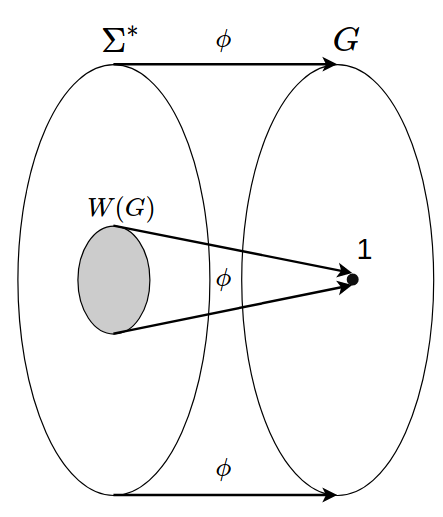
\includegraphics[width=0.6\linewidth]{pics/3.png}}
\caption{Word problem of group.}
\label{fig:word_problem}
\end{figure}

In the following, we present one-tape machine commands that as result replace \eqref{eqreplace},
insert \eqref{eqinsert}, move to left \eqref{eqmove} and delete \eqref{eqdelete} squares.
\begin{equation}
    u q v \to u' q' v' \label{eqreplace}
\end{equation}
\begin{equation}
    q \omega \to u q' \omega \label{eqinsert}
\end{equation}
\begin{equation}
    u q \to q' u \label{eqmove}
\end{equation}
\begin{equation}
    u q \omega \to q' \omega \label{eqdelete}
\end{equation}
where $u$, $v$, $u^'$, $v^'$ are letters or empty words.  

Also, we need to mention a class of machines called symmetric Turing machines.
\begin{defn}
Turing machine is symmetric if for every command in the set of commands there 
is its inverted command.
\end{defn}
For  example, for command 
$u q v \to u' q' v'$ the inverted command is $u' q' v' \to u q v$.

In addition, authors introduce absolutely new definition called S-machines and defined it as rewriting systems.

\begin{defn}
Let $n$ be a natural number. 
A hardware of an S-machine is a pair $(Y, Q)$ where 
\begin{itemize}
    \item $Y$ is a $n$-vector of sets $Y_i$ which elements are called tape letters.
    \item $Q$ is a $(n + 1)$-vector of disjoint sets $Q_i$ which elements are called state letters.
\end{itemize}
The sets of elements of $Q$ and $Y$ are also disjoint. 
\end{defn}

With every hardware $S = (Y, Q)$ can be associate the language of admissible words 
$L(S) = Q_1F(Y_1)Q_2 \dots F(Y_n)Q_{n+1}$ where $F(Y_j)$ is the language 
of all reduced group words in the alphabet $Y_j \cup Y_j^{-1}$.

The rewriting rules, or S-rules, have the following form:
$[U_1 \to V_1, \dots ,  U_m \to V_m]$
where the following conditions hold:
\begin{enumerate}
    \item Each $U_i$ is a subword of an admissible word starting with a $Q_l$-letter and ending with a $Q_r$-letter.
    \item If $i < j$ then $r(i) < l(j)$.
    \item Each $V_i$ is also a subword of an admissible word whose $Q$-letters belong to $Q_{l(i)} \cup \dots \cup Q_{r(i)}$ and which contains a letter from $Q_l$ and and from $Q_r$.
    \item Tape letters are not inserted to the left of $Q_1$-letters and to the right of $Q_{n+1}$-letter.
\end{enumerate}

To apply an S-rule to a word $W$ means to replace simultaneously 
subwords $U_i$ by subwords $V_i$, $i = 1, \dots, m$. After every application of 
a rewriting rule, the word is automatically reduced.

For example, if a word is 
$q_1 a a q_2 b q_3$ 
and the S-rule is 
$\newline
[q_1 \to p_1 a^{-1}, q_2 b q_3 \to a^{-1} p_2 b' q_3] $
where $q_i \in Q_i$, $p_i \in Q_i$, $a \in Y_1$, $b, b' \in Y_2$ then the result 
of the application of this rule is
$p_1 p_2 b' q_3$.

Besides, with every S-rule $\tau$ we need to associate the inverse S-rule $\tau^{-1}$ in the following way: if  
$\\ \tau = [U_1 \to x_1 V_1 y_1, \dots, U_m \to x_m V_m y_m]$
then
$\\ \tau^{-1} = [V_1 \to x_1^{-1} U_1 y_1^{-1}, \dots, V_m \to x_m^{-1} U_m y_m^{-1}]$

It is worth noting that throughout their work, the authors assume that 
an S-machine is symmetric; i. e. if an S-machine contains 
a rewriting rule $\tau$, it also contains the rule $\tau^{-1}$.

\begin{thm} \label{thmTM}
For any Turing machine $ M $ that recognizes the language $ L $, there is
Turing machine $ M' $ with the following properties:
\begin{itemize}
\item The language that $ M'$ recognizes is $ L $.
\item $ M'$ is symmetric.
\item A machine accepts a word only when all tapes are empty.
\item Any command $ M' $ or its inverse has one of the following forms for some i:
\begin{enumerate}
\item $\{ q_1 \omega \to q'_1 \omega, \dots, q_{i-1} \omega \to q'_{i-1} \omega, \\
a q_i \omega \to q'_i \omega, q_{i+1} \omega \to q'_{i+1} \omega, \dots \}$
\item $\{q_1 \omega \to q'_1 \omega, \dots, q_{i-1} \omega \to q'_{i-1} \omega, \\
\alpha q_i \omega \to \alpha q'_i \omega, q_{i+1} \omega \to q'_{i+1} \omega, \dots \} $
\end{enumerate}
where $a$ belongs to the tape alphabet of the tape $i$, and $q_j, q'_j$ are the 
states of the tape $j$.
\item The letters used on different tapes, including states, belong to non-overlapping alphabets.
\end{itemize}
\end{thm}

We note that symmetric Turing machines are more similar than usual to a group 
because of the possibility of inverse computations that are possible in a group. 
The proof of this theorem allows us to construct a symmetric Turing machine 
while preserving the recognizable language of the original machine.

In the next step, the authors propose to build an S-machine from a symmetric 
Turing machine to achieve even greater similarity with the groups. 
There is a “natural” way of transforming a Turing machine into an S-machine. 
For this, we take a Turing machine $ M $ satisfying all the conditions of Theorem 2,
combine all the tapes of the machine $ M $ and replace each command 
$a q \omega \to q' \omega$
on $q \omega \to a^{- 1} \omega$, so the $ M $ commands become S-rules.
Unfortunately, an S-machine constructed in this way does not inherit most 
of the properties of the original M machine. This is because the S-machine 
alphabet contains inverse characters.

Before starting to build an S-machine, the authors make the following renames. 
For every $q \in Q$ they denote the word $q \omega$ by $F_q$ and the left marker 
on tape $# i$ by $E_i$.
Besides, for any configuration $ C = (E_1 u_1 F_{q_1}, ..., E_k u_k F_{q_k}) $
of the machine $ M $, they introduce
the value of $\sigma(C)$, which is the admissible word for $S(M)$:

\begin{IEEEeqnarray}{lCr}
E(0)\alpha^n x(0)F(0) \nonumber \\
E(1)u_1x(1)F_{q_1}(1)E'(1)p(1)\delta^{||u_1||}q(1)r(1)s(1)t(1) \nonumber \\
\overline{p}(1)\overline{q}(1)\overline{r}(1)\overline{s}(1)
\overline{t}(1)F'_{q_1}(1) \nonumber \\
... \nonumber \\
E(k)u_k x(k)F_{q_k}(k)E'(k)p(k)\delta^{||u_k||}q(k)r(k)s(k)t(k) \nonumber \\
\overline{p}(k)\overline{q}(k)\overline{r}(k)\overline{s}(k)
\overline{t}(k)F'_{q_k}(k) \nonumber \\
E'(k + 1)x(k + 1)\omega^n F'(k + 1) \nonumber
\end{IEEEeqnarray}
where $n = |u_1| + ... + |u_k|$.

Then the following theorem states that for any Turing machine satisfying Theorem \ref{thmTM}, 
there is an S-machine simulating it.

\begin{thm} \label{thmsm}
Let $ M = \langle X, Y, Q, \Theta, s_1, s_0 \rangle $ be a Turing machine,
which satisfies the conditions of Theorem \ref{thmTM}.
Let $W_0 = \sigma(C_0)$, where $C_0$ is start configuration of the Turing machine $M$.
Then the configuration $ C $ of the machine $ M $ is admissible for $M$ if
and only if $ S (M) $ can transfer $ \sigma(C) $ to $ W_0 $ by rewriting rules.
\end{thm}

At the last step of transforming, the authors finally build the group. 
Note that they call one of each pair of mutually inverse rules from $\Theta$ 
positive and the other negative. 
The set of all positive rules is denoted by $\Theta^+$, and the set of 
all negative rules is denoted by $\Theta^-$.

\begin{thm}
Let $S(M)$ be the S-machine described in Theorem \ref{thmsm}, 
then for any positive integer $N$, 
there exists a representation of the group $ G_N (S) $ 
with the generated set $ A $ and with the set of relations $ P_N (S) $, 
where
$\\
A = \cup^{17k+6}_{i=1} Q_i \cup \{\alpha, \omega, \delta\} 
\cup \cup^k_{i=1}Y_i \cup \{k_j | j = 1, \dots, 2N\} \cup \Theta^+$
and the set of relationships consists of the following:
\begin{enumerate}
\item Transition relations.

These relations correspond to elements of $ \Theta^+$.
Let $ \tau \in \Theta^+, \tau = [U_1 \to V_1, ..., U_p \to V_p] $.
Then we include the relations $ U^{\tau}_1 = V_1, ..., U^{\tau}_p = V_p $.
If for some $j$ from 1 to $17k + 6$, letters from $Q_j$ do not appear in any of the $U_i$, 
then also include the relations $ q^{\tau}_j = q_j $ for each $ q_j \in Q_j $.
\item Auxiliary relations.

This is all kinds of relations of the form $\tau x = x \tau $, where
$ x \in \{\alpha, \omega, \delta \} \cup^k_{i = 1} Y_i, \tau \in \Theta^+ $ and all relations 
of the form $ \tau k_i = k_i \tau, i = 1, ..., 2N, \tau \in \Theta^+ $.
\item The hub relation.

Let for each word $u$ $K(u)$ denote the word \eqref{eqku}.
\begin{IEEEeqnarray}{rCl}
K(u) &=& (u^{-1} k_1 u k_2 u^{-1} k_3 u k_4 ... u^{-1} k_{2N-1} u k_{2N}) \nonumber \\ 
&& {} \cdot (k_{2N} u^{-1} k_{2N-1} u ... k_2 u^{-1} k_1 u)^{-1} \label{eqku}
\end{IEEEeqnarray}

Then the hub relation is $K(W_0) = 1$.
\end{enumerate}
\end{thm}

The authors described and proved all the constructions in the theorems above, 
but no one has automated these constructions at the moment, 
which we are trying to do in this work.

Using this information, we are ready to introduce the main theorem of the considered article. 

\begin{thm}
Let $L \subseteq \Sigma^+$ be the language accepted by the Turing machine $M$, then there exists a finitely presented group $G(M) = \langle A ~ | ~ R \rangle$ and the injective mapping
$\\K: \Sigma^+ \to (A \cup A^{-1})^+$ such that: $\\u \in L \iff K(u) \in W(G) $
\end{thm}

\section{Implementation}

This section provides a brief description of the algorithm for constructing 
a group presentation by a formal context-free grammar. 

The first part of the algorithm does not connect to the article discussed in the previous section and faced to bridge a gap between context-free grammar and the Turing machine. 
To achieve that we implement pushdown automata in terms of the Turing machine we introduced
in the background. The algorithm accepts a formal grammar in Chomsky normal form as input, 
it is necessary for ease implementation of pushdown automation.
As we mentioned earlier in Theorem \ref{thmpda}, it allows 
us to recognize context-free languages and in the end, 
we can construct groups presentation of 
up to context-free languages. It means at this moment we cannot transform wider 
classes e.g. recursively enumerable languages, which can be recognized 
by the Turing machine, but narrower one can be transformed. 

Another part of the algorithm consists of several separate steps, 
which can be seen in Fig. \ref{fig:sheam}. 
It depicts a diagram of successive transformations that translate 
a Turing machine \textit{TM} into a presentation of a group \textit{G} 
with an injective mapping \textit{K} that translates a language recognized by 
a Turing machine \textit{TM} into a word problem of a group \textit{G}. 
To implement these transformations, we analyzed the proofs 
of the theorems presented above and based on them we developed the algorithm. 

Besides, we use the Haskell functional programming 
language\footnote{\url{https://github.com/YaccConstructor/LangToGroup}}, 
this choice was due to its rich and convenient type system, 
which we apply to represent algorithmic types such as formal grammar, 
Turing machine, S-machine or group. The program was divided into modules 
that coincide in meaning and content with the blocks and transitions 
in Fig. \ref{fig:sheam}. Moreover, to facilitate the process of developing 
and testing the algorithm, debug printing of types in LaTeX was implemented.

\begin{figure}[bp]
\centerline{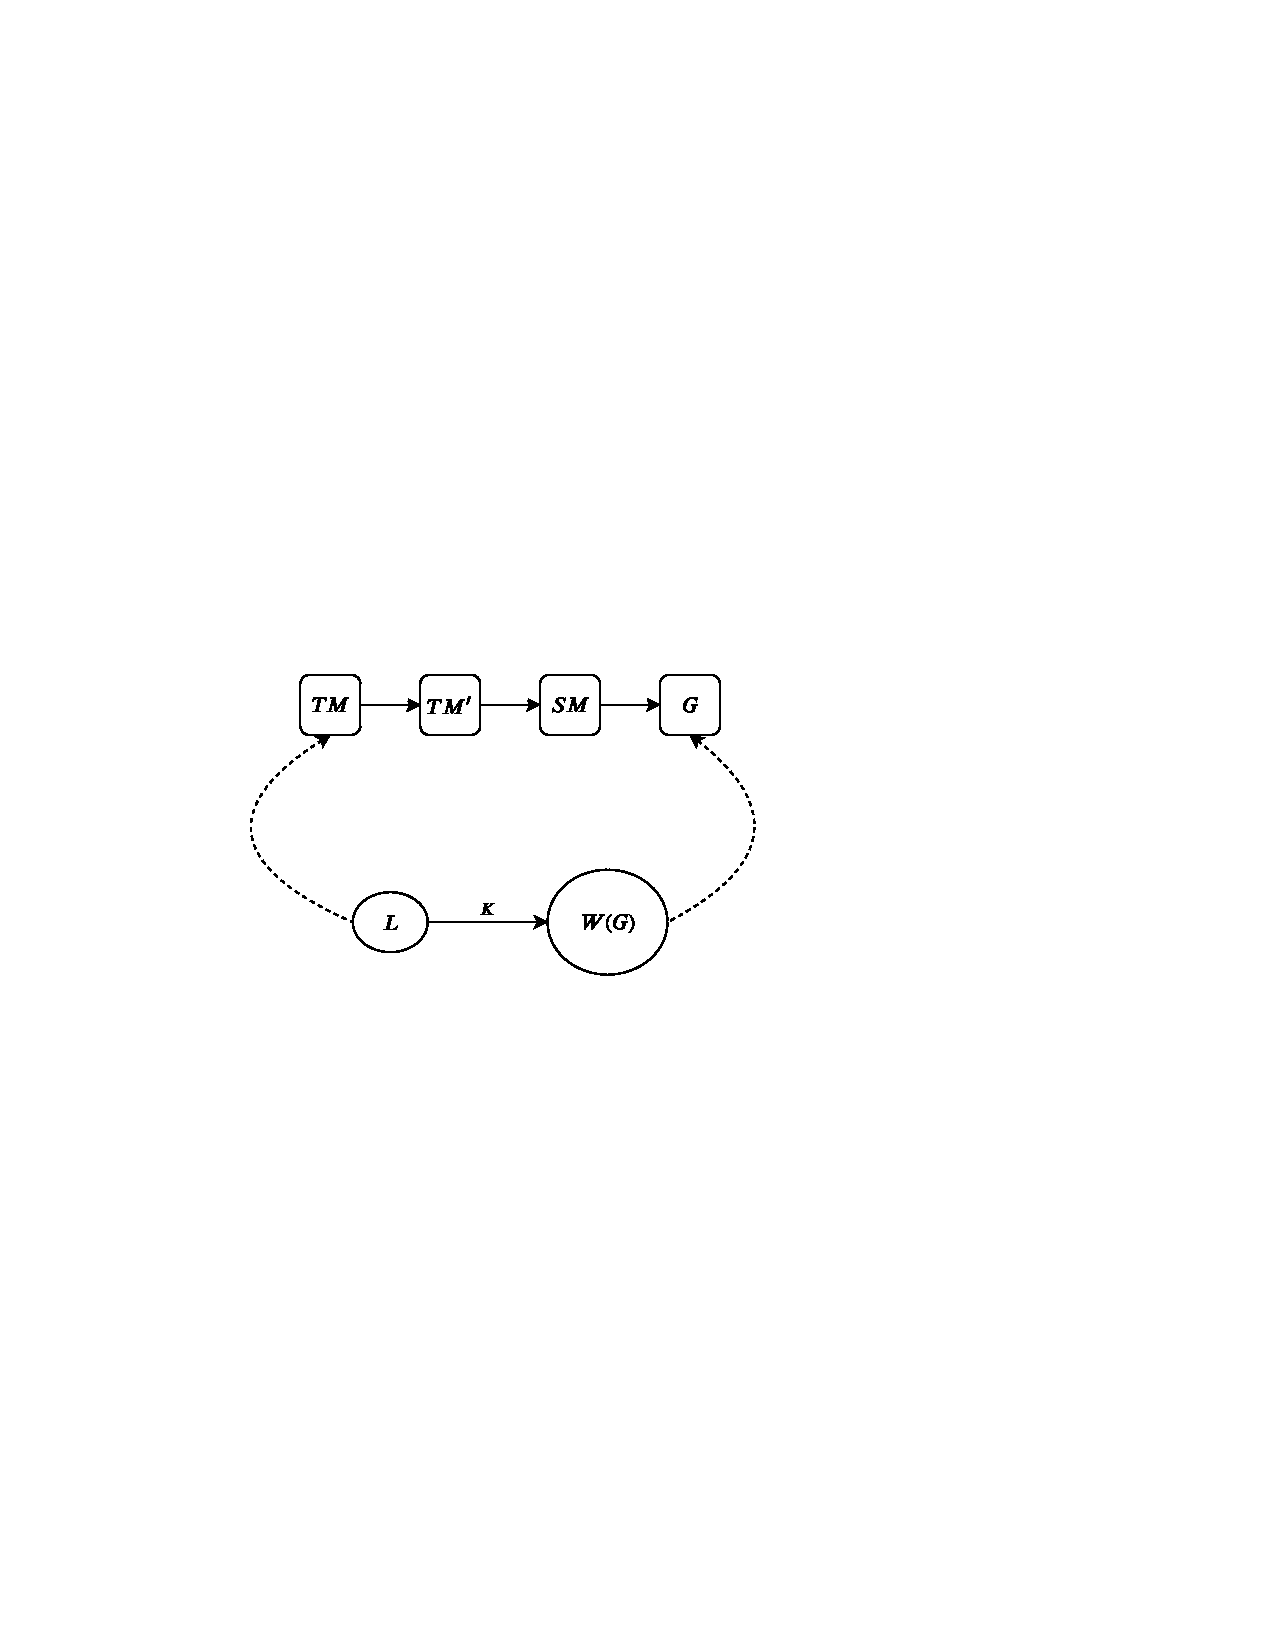
\includegraphics[width=\linewidth]{pics/2.pdf}}
\caption{Transformation diagram.}
\label{fig:sheam}
\end{figure}

\section{Evaluation}

\begin{table*}[tp]
\begin{center}
\begin{tabular}{|c!{\vrule width 1pt}
c|c|c!{\vrule width 1pt}
c|c|c|c!{\vrule width 1pt}
c|c|c|c!{\vrule width 1pt}
c|c|c!{\vrule width 1pt}
c|c!{\vrule width 1pt}}
\hline
&
\multicolumn{3}{|c|}{\textbf{Grammar}}&
\multicolumn{4}{|c|}{\textbf{TM}}&
\multicolumn{4}{|c|}{\textbf{TM'}}&
\multicolumn{3}{|c|}{\textbf{SM}}&
\multicolumn{2}{|c|}{\textbf{G}}\\
\cline{2-17} 
&$\Sigma$&$N$&$R$ 
&$X$&$\Gamma$&$Q$&$\Theta$  
&$X$&$\Gamma$&$Q$&$\Theta$
&$Y$&$Q$&$\Theta$
&$A$&$R$\\
\hline
1 rule 
&1&1&1 
&1&3&6&5 
&1&16&548&232
&16&178042&2615
&180678&68855\\
\hline
$a^*$ 
&1&2&3 
&1&4&8&11 
&1&30&1166&500
&30&772234&6557
&778826&263305\\
\hline
Dyck 
&2&4&6 
&2&8&13&20 
&2&56&2068&898
&56&2431326&14253
&2445640&940205\\
\hline
\end{tabular}
\end{center}
\caption{Number of elements in the sets.}\label{tab:1}
\end{table*}

We evaluate the implementation described above on three grammars: one rule grammar \eqref{eqonerule},
"a" star language grammar \eqref{eqastar}, and Dyck language grammar \eqref{eqdyck}. 

\begin{multicols}{2}
\noindent
\centering
    \begin{IEEEeqnarray}{lCr}
        \nonumber \\ S \to a \label{eqonerule}    
    \end{IEEEeqnarray}
    \begin{IEEEeqnarray}{lCr}
        S \to AS \nonumber \\
        S \to \epsilon \label{eqastar} \\
        A \to a \nonumber
    \end{IEEEeqnarray}
    \begin{IEEEeqnarray}{lCr}
        S \to AC \nonumber \\
        S \to \epsilon \nonumber \\
        C \to SD \label{eqdyck} \\
        D \to BS \nonumber \\
        A \to a \nonumber \\
        B \to b \nonumber
    \end{IEEEeqnarray}
\end{multicols}

Table \ref{tab:1} shows the sizes of each of the sets of our algebraic data structures. 
It is clear, that we got the algorithm that even on simple initial data gives 
an immense group presentation. So, only one grammar rule turns into 68855 
group relations and the number of generators also increased dramatically. 
But if we take a closer look, we will see that the main explosion occurs 
at the step of transforming the symmetric Turing machine into an S-machine. 
This means that, if we want to get a presentation of a group of satisfying sizes, 
then in future work we need to learn, how to convert symmetric Turing machines 
into S-machines in a more optimal way. 

Because the final algorithm turned out difficult its can not be tested as usual 
using unit tests, and a series of experiments were carried out in an attempt 
to prove the correctness of the algorithm, but because of the computational complexity, 
the mathematical packages with which the experiments were carried out did not complete 
their work for a long time and did not confirm the correctness of the algorithm.

\section{Conclusion}

During this work, an algorithm for constructing a group presentation 
using a Turing machine was implemented and several experiments were 
carried out that were unsuccessful.

On the other hand, other methods for constructing an S-machine 
using a symmetric Turing machine have already been described 
(see, for example, \cite{SpaceFunc}), and this step, as we said earlier, 
is the bottleneck of the described algorithm. 
Therefore, it makes sense in future work to implement other constructions 
of S-machines, to check their quality factor.

At this point, the work still in progress, we try to find an appropriate 
way to confirm or modify our algorithm.

\bibliographystyle{IEEEtran.bst}
\bibliography{IEEEbib.bib}
\end{document}
